% !TEX root = ../Diplombericht.tex
\subsection{Physikalischer Überblick}
Die nachfolgende Abbildung stellt ein verinfachter Überblick der vorgesehenen Infratstruktur dar.

\begin{figure}[htb]
\centering
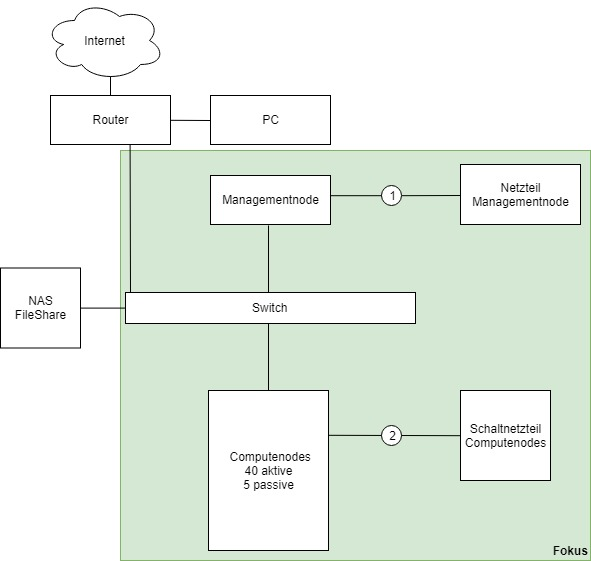
\includegraphics[scale=0.5]{phys_ueberblick.jpg}
\caption{Physikalischer Überblick}
\label{fig:Physikalischer Überblick}
\end{figure} 

\textbf{Beschreibung}\newline
Der grün markierte Teil beinhaltet das Vorhaben. Diese Komponenten werden neu in das Netzwerk eingebunden und aufgebaut. Die Komponenten ausserhalb des grünen Bereiches existieren bereits und es müssen für die Umsetzung konfigurationen vorgenommen werden.

\textbf{Verbindung 1} \newline
Der Managementnode wird über ein herkömmliches Netzteil per Micro USB mit Stom versorgt.

\textbf{Verbindung 2} \newline
Die Computenodes werden über ein Schaltnetzteil über die GPIO Pins mit Stom betrieben.


\subsubsection{Technischer Überblick}

\begin{figure}[H]
\centering
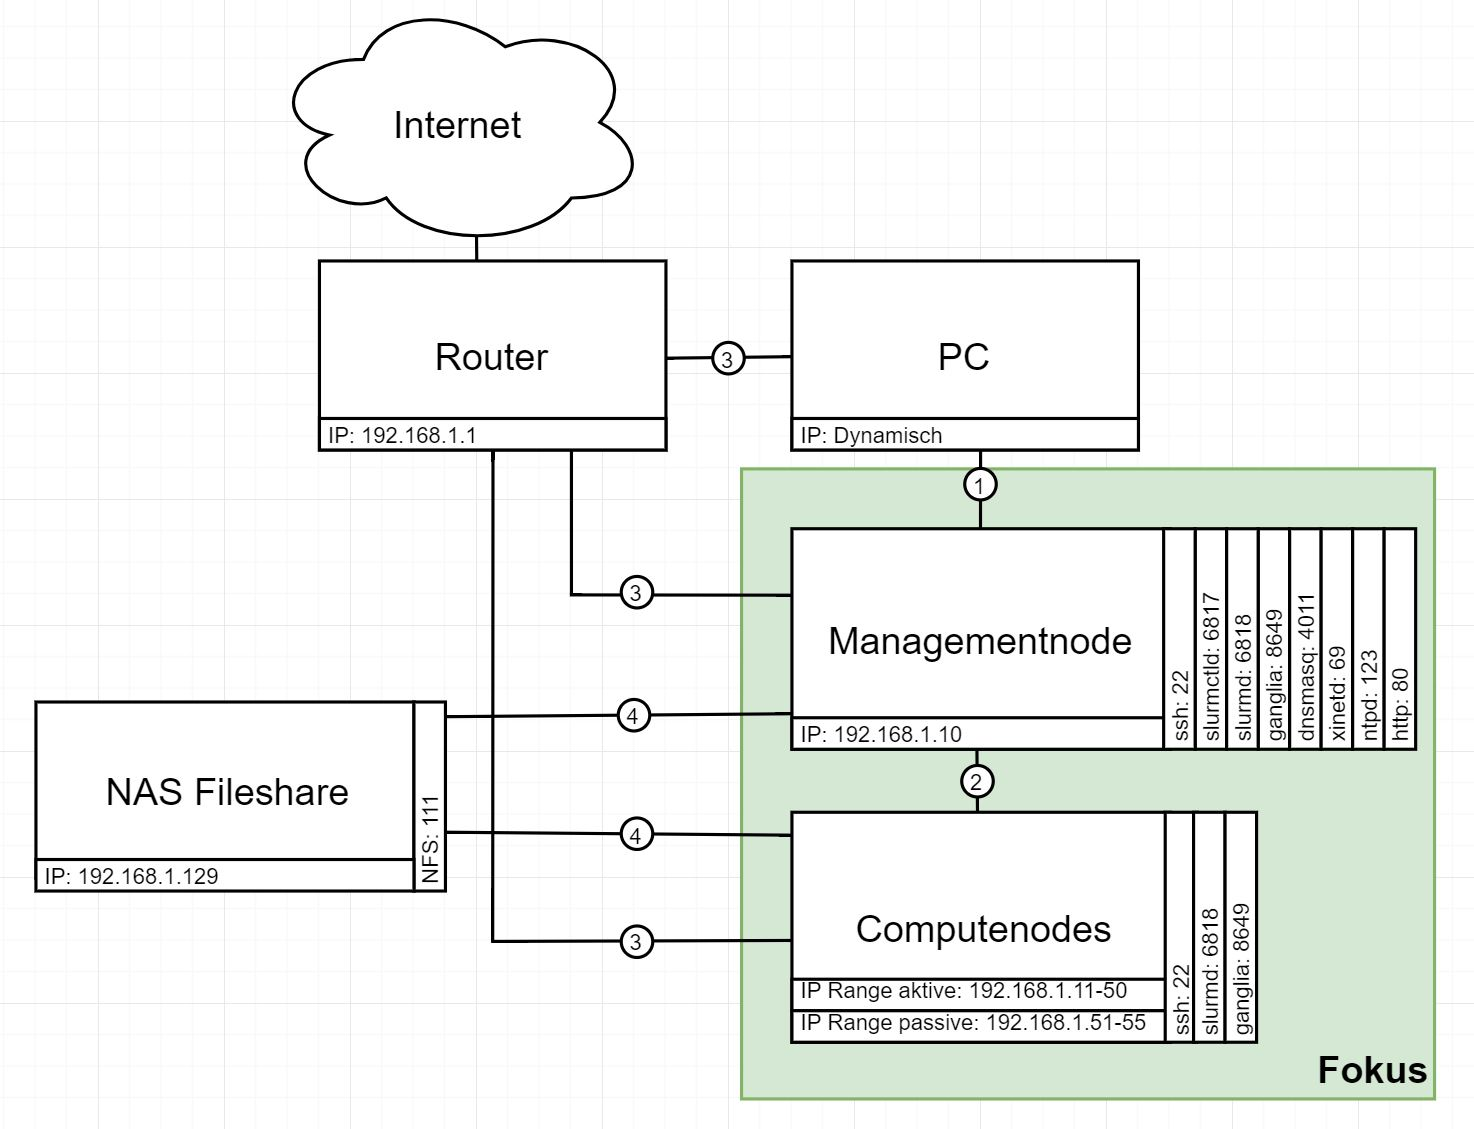
\includegraphics[scale=0.5]{tech_ueberblick.jpg}
\caption{Technischer Überblick}
\label{fig:Technischer Überblick}
\end{figure} 


\begin{table}[H]
\centering
\begin{tabular}{p{1cm}p{5cm}p{5cm}p{5cm}}
\hline
\rowcolor{heading} \textbf{Verbindung} & \textbf{Protokoll} & \textbf{Protokollfamilie} & Ports \\\hline
1 & SSH & TCP & 22 \\\hline
2 & SMB & TCP & 445 \\\hline
3 & DHCP & UDP & 67 / 78 \\\hline
4 & TFTP & UDP & 69 \\\hline
5 & HTTP & TCP & 80 \\\hline
\end{tabular}
\caption{Protokolle}
\end{table}
